
\begin{enumerate}
\item The feasible set is shown on the Figure below.


\begin{center}

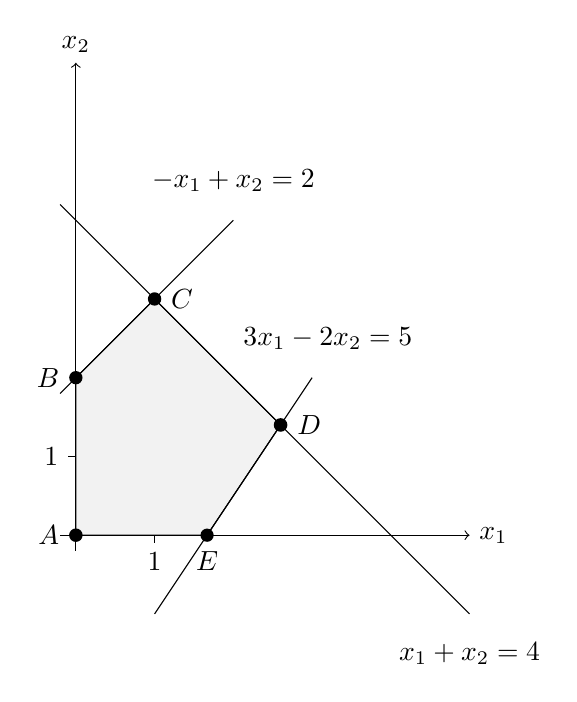
\begin{tikzpicture}[transform shape]%[domain=-0.3:15.5,range=-0.5:14]
       \draw[fill=lightgray!20]  (0,0) -- (0,2) -- (1,3) -- (13/5,7/5) -- (5/3,0) -- cycle;

      \draw (0,1) -- (-0.1,1) node[left] {1} ;
      \draw (1,0) -- (1,-0.1) node[below] {1} ;
      \draw[->] (-0.2,0) -- (5,0) node[right] {$x_1$};
      \draw[->] (0,-0.2) -- (0,6) node[above] {$x_2$};

   \node[circle,fill=black, label=left:$A$,scale=0.25] at (0,0) {A};
   \node[circle,fill=black, label=left:$B$,scale=0.25] at (0,2) {B};
   \node[circle,fill=black, label=right:$C$,scale=0.25] at (1,3) {C};
   \node[circle,fill=black, label=right:$D$,scale=0.25] at (13/5,7/5) {D};
   \node[circle,fill=black, label=below:$E$,scale=0.25] at (5/3,0) {E};
      
      \draw[color=black] (-0.2,1.8) -- (2,4);
      \node at (2,4.5) {$-x_1 + x_2 = 2$};
      
       \draw[color=black] (1,-1) -- (3,2);
       \node at (3.2,2.5) {$3x_1 -2 x_2 = 5$};
      
      \draw[color=black] (-0.2,4.2) -- (5,-1);
      \node at (5,-1.5) {$x_1+x_2=4$};
      
       
  

\end{tikzpicture} 

\end{center}

The set of vertices is
\[
\begin{array}{cll}
  & (x_1,x_2) & -3x_1 - 4 x_2 \\
  \hline
  A & (0,0) & 0 \\
  B & (0,2) & -8 \\
  C & (1,3) & -15 \\
  D & (13/5,7/5) & -13.4 \\
  E  & (5/3,0) & -5.
\end{array}
\]
  Calculating the objective function at each vertex,
we obtain that $C(1,3)$ is optimal with optimal value -15. Note that,
at the optimal solution the constraints
\begin{align*}
-x_1+x_2 & \leq 2,\\
x_1+x_2 & \leq 4,\\
\end{align*}
are active, while the constraint
\[
-3x_1+2x_2  \geq -5
\]
is not. 


\item Using the summary tables, we obtain the dual problem:
\[
\max 2\gamma_1-5\gamma_2+4\gamma_3
\]
subject to 
\begin{align*}
-\gamma_1-3\gamma_2+\gamma_3 & \leq -3,\\
\gamma_1+2\gamma_2+\gamma_3 & \leq -4,\\
\gamma_1 & \leq 0,\\
\gamma_2 & \geq 0,\\
\gamma_3 & \leq 0.
\end{align*}

\item By complementarity slackness, as the second constraint is not active, the corresponding
dual variable must be zero: $\gamma^*_2=0$.
Also, as the two primal variables are non zero, the
  corresponding dual constraints must be active, and we have the following
  equations:
\begin{align*}
-\gamma^*_1-3\gamma^*_2+\gamma^*_3 & = -3,\\
\gamma^*_1+2\gamma^*_2+\gamma^*_3 & = -4.\\
\end{align*}
Putting the two together, we have
\begin{align*}
-\gamma^*_1+\gamma^*_3 & = -3,\\
\gamma^*_1+\gamma^*_3 & = -4,\\
\end{align*}
so that the optimal solution of the dual is
\begin{align*}
  \gamma_1^* &= -1/2, \\
  \gamma_2^* &= 0, \\
  \gamma_3^* &= -7/2. \\
\end{align*}
The optimal value is
\[
2\gamma^*_1-5\gamma^*_2+4\gamma^*_3 = -1-14= -15,
\]
 as expected from the strong duality theorem.

\end{enumerate}

